\documentclass{article}
\usepackage[utf8]{inputenc}
\usepackage{amsmath, amsthm, amssymb}
\usepackage{graphicx}
\usepackage{algorithm}
\usepackage{algpseudocode}
\usepackage{listings}
\usepackage{xcolor}
\usepackage[export]{adjustbox}

\definecolor{codegreen}{rgb}{0,0.6,0}
\definecolor{codegray}{rgb}{0.5,0.5,0.5}
\definecolor{codepurple}{rgb}{0.58,0,0.82}
\definecolor{backcolour}{rgb}{0.95,0.95,0.92}

\lstset{
    language=Python, 
    basicstyle=\ttfamily\small,
    commentstyle=\color{codegreen},
    keywordstyle=\color{magenta},
    numberstyle=\tiny\color{codegray},
    stringstyle=\color{codepurple},
    breakatwhitespace=false,         
    breaklines=true,                 
    captionpos=b,                    
    keepspaces=true,                 
    numbers=left,                    
    numbersep=5pt,                  
    showspaces=false,                
    showstringspaces=false,
    showtabs=false,                  
    tabsize=2,
    frame=single,
    backgroundcolor=\color{white}
}

\title{A Lock-Free Interaction Combinator Evaluator}
\author{Victor Taelin}
\date{}

\begin{document}

\maketitle

\begin{abstract}
We present a lock-free evaluator for interaction combinators, a simple yet powerful model of distributed computation. The proposed algorithm is based on the concept of implicit ownership regions and redirectors, allowing for efficient parallel evaluation without race conditions or deadlocks. We provide detailed illustrations, and the pseudocode for the core procedures can be found in the appendix. We have implemented our lock-free evaluator in CUDA and achieved successful reductions of large graphs on GPUs with thousands of concurrent threads, demonstrating the practicality and efficiency of our approach.
\end{abstract}

\section{Introduction}\label{s:introduction}

Interaction nets are a graphical model of computation designed as a generalization of the proof structures of linear logic~\cite{girard1987linear}. They consist of graph-like structures composed of agents and edges, where each agent has a type and an arity connected to other agents via its ports. Interaction nets are inherently distributed, allowing computations to take place simultaneously in many parts of a net without synchronization. This makes them suitable for modeling massive parallelism.

A specific type of interaction nets is the system called \textit{interaction combinators}, introduced by Lafont~\cite{lafont1997interaction}. These are built from three types of nodes: constructor (CON), duplicator (DUP), and eraser (ERA). Each node has a principal port and two auxiliary ports. The nodes interact according to six rules, divided into two categories: commutation and annihilation. Commutation rules apply when two different types of nodes are connected through their principal ports, while annihilation rules apply when two nodes of the same type are connected through their principal ports. In this paper, we use the symmetric interaction combinator variant, which has been described by Mazza~\cite{mazza2007denotational}, and is illustrated below:

\begin{figure}[h!]
\centering
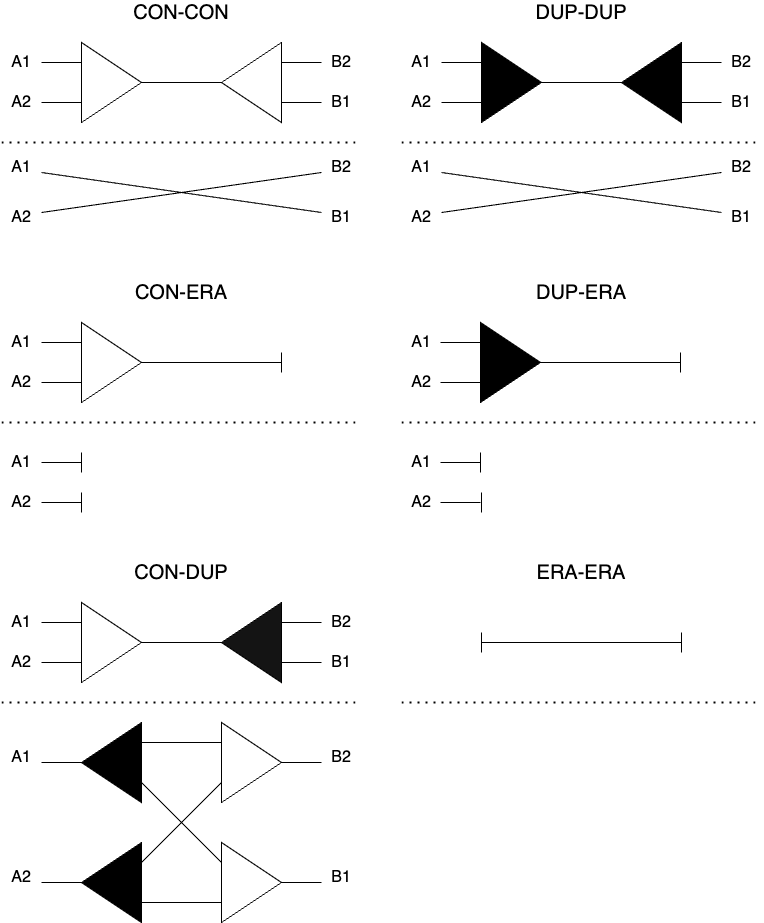
\includegraphics[width=1.0\textwidth,margin=4 4 4 4]{interaction_rules.png}
\caption{Interaction rules}
\end{figure}

Interaction combinators possess several key properties such as determinism, locality, strong confluence (diamond property), and universality. These properties make them particularly suitable for modeling distributed and parallel computations~\cite{lafont1997interaction}. Yet, despite that theoretical appeal, there has been limited practical exploration of their potential for massive parallel computation on modern hardware. In this paper, we propose a lock-free evaluator for interaction combinators that achieves near-ideal speedup on modern GPUs, with several thousand concurrent threads. The heart of our implementation is a lock-free \texttt{link()} procedure, which we describe in detail.

The paper is organized as follows: Section 2 discusses the limitations of a lock-based evaluator. Section 3 introduces our proposed lock-free evaluator. Section 4 presents an optimization to further increase parallelism. Section 5 discusses the implementation details and the performance of our CUDA-based evaluator~\cite{taelin2022lock}. Finally, Section 6 concludes the paper and discusses future work.

\section{Former Work}\label{s:former_work}


A lock-based evaluator for interaction nets was developed by Sato et al. in their work on Inpla: Interaction Nets as a Programming Language~\cite{hassan2010implementation, sato2014implementation}. Inpla is a multi-threaded parallel interpreter for interaction nets that aims to provide efficient execution of programs in both sequential and parallel environments. Inpla, based on the Lightweight calculus, focuses on the representation, calculus, data structures, and low-level language for implementing interaction nets. Their approach involves using compare-and-swap atomic operations and locking mechanisms, which can be sub-optimal when dealing with parallelism. The locking mechanisms used in Inpla can potentially lead to performance bottlenecks, especially when the checking process for locks spreads globally across the net.

Another approach, the ingpu evaluator~\cite{jiresch2014towards} was introduced as a GPU-based implementation of interaction nets. The ingpu evaluator, implemented using the CUDA/Thrust library, focused on the interaction and communication phases of the lightweight interaction calculus rather than maintaining an array of redexes and performing explicit graph rewrites. However, the ingpu method faced performance bottlenecks due to sorting and merging arrays, difficulty in representing the irregular graph structure, and varying output size of a reduction.

\section{Lock-Based Evaluator}\label{s:lockfree}

The naive approach to reducing interaction combinators in parallel is to represent nets as vectors of nodes, with ports holding pointers to their destinations, and maintain a set of redexes (active pairs) to process concurrently. However, this can lead to race conditions due to overlapping regions. To address this, the affected regions, which include two active nodes and up to 4 surrounding nodes, must be locked. This approach is illustrated below:

\begin{figure}[h!]
\centering
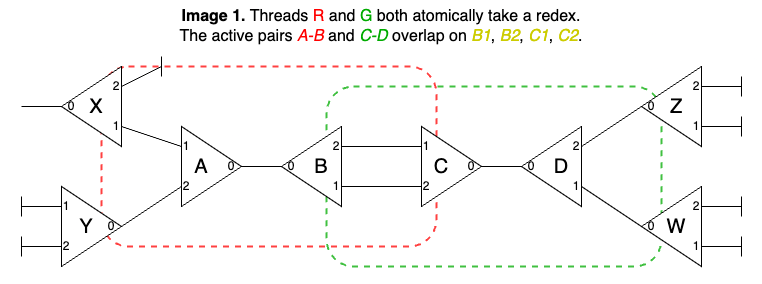
\includegraphics[width=1.0\textwidth,margin=4 4 4 4]{lock_based_evaluator_1.png}
\caption{Lock-based evaluator step 1}
\end{figure}

\begin{figure}[h!]
\centering
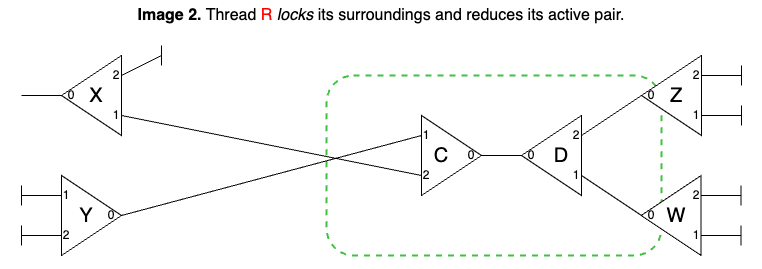
\includegraphics[width=1.0\textwidth,margin=4 4 4 4]{lock_based_evaluator_2.png}
\caption{Lock-based evaluator step 2}
\end{figure}

\begin{figure}[h!]
\centering
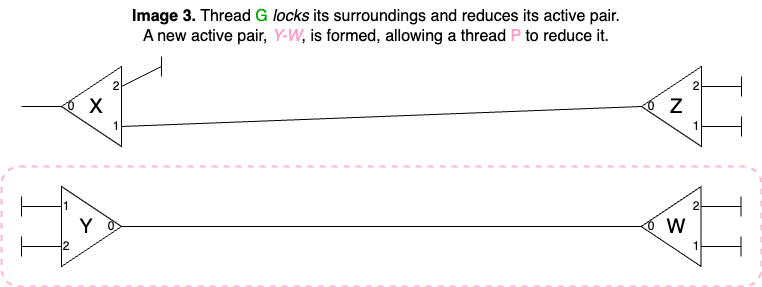
\includegraphics[width=1.0\textwidth,margin=4 4 4 4]{lock_based_evaluator_3.png}
\caption{Lock-based evaluator step 3}
\end{figure}

While this strategy works, locking the 6 surrounding nodes can be challenging, potentially leading to a deadlock. For example, consider thread R locking active nodes A and B, while thread G locks active nodes C and D. To proceed with the reduction, thread R must lock C, and thread G must lock B, which is impossible in this situation.

To avoid deadlocks, one could attempt to lock nodes in an established order, such as from left to right. This prevents deadlocks but may cause a thread to lock an irrelevant region. For instance, suppose thread R locks X and Y immediately before another thread reduces the X node, replacing it with K. Thread R then locks A, B, and C, incorrectly locking the region X, Y, A, B, and C, instead of including the new node K. Consequently, thread R cannot proceed with its reduction.

Any viable solution to this issue will inevitably involve back-offs or temporary deadlocks, causing the algorithm to rely on the scheduler. This dependence can have negative implications for performance, particularly in architectures such as GPUs, where warps operate in lockstep. The tight synchronization in such systems can exacerbate performance issues, leading to less efficient execution of the algorithm.

\section{Lock-Free Evaluator}\label{s:lockfree}

In this section, we propose an efficient lock-free reduction algorithm based on implicit ownership regions and redirection wires. The idea is to process a set of redexes in parallel, but perform rewrites only within implicitly owned regions, eliminating the need for locks.

When a thread obtains a redex, it assumes ownership of its two active nodes. It then replaces these nodes with redirection wires, allowing the redex to be semantically reduced without affecting the surrounding region. Next, the thread expands its ownership region to include surrounding nodes connected to it via main ports. Finally, the thread invokes a linking procedure that starts from these surrounding main ports and traverses the graph, clearing redirection wires until arriving at a port outside its ownership region. At this point, there are two cases to consider:

1. If the outside port is an auxiliary port, the thread attempts to connect the surrounding main port to it using an atomic compare-exchange operation and clears the backward path.

2. If it is a main port, the thread has found a new active pair and coordinates with the opposing thread — which will traverse the backward path — to create a new redex.

The following illustrations showcase this process:

\begin{figure}[h!]
\centering
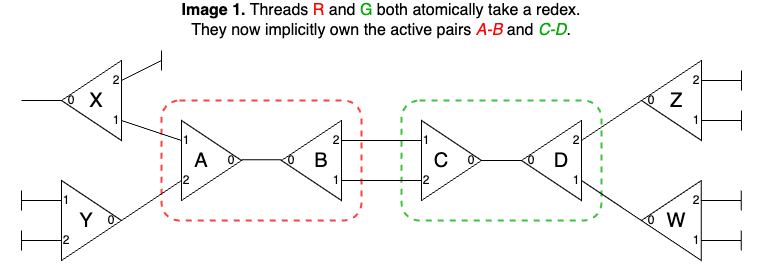
\includegraphics[width=1.0\textwidth,margin=4 4 4 4]{lock_free_evaluator_1.png}
\caption{Lock-free evaluator step 1}
\end{figure}

\begin{figure}[h!]
\centering
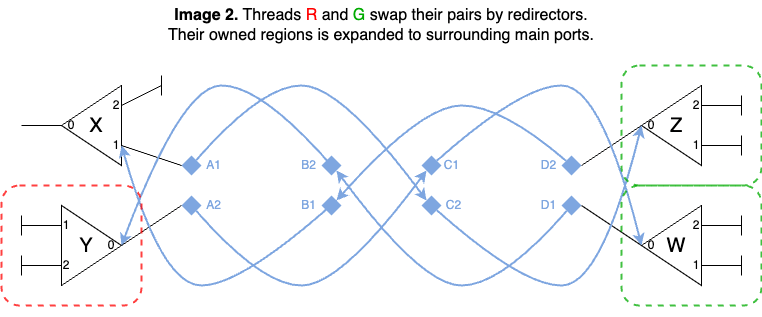
\includegraphics[width=1.0\textwidth,margin=4 4 4 4]{lock_free_evaluator_2.png}
\caption{Lock-free evaluator step 2}
\end{figure}

\begin{figure}[h!]
\centering
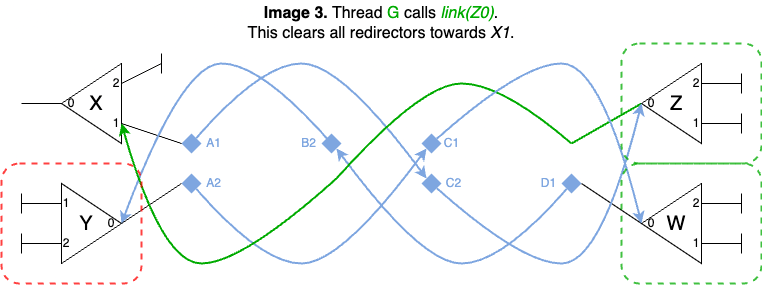
\includegraphics[width=1.0\textwidth,margin=4 4 4 4]{lock_free_evaluator_3.png}
\caption{Lock-free evaluator step 3}
\end{figure}

\begin{figure}[h!]
\centering
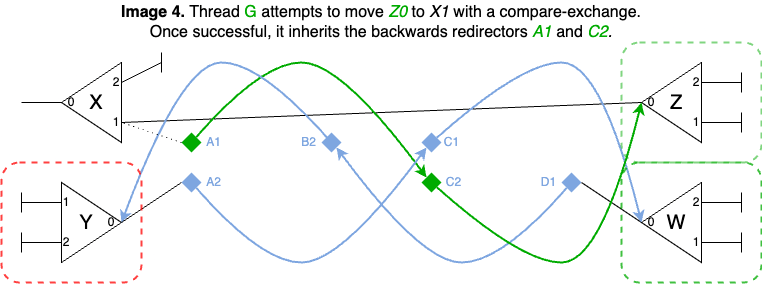
\includegraphics[width=1.0\textwidth,margin=4 4 4 4]{lock_free_evaluator_4.png}
\caption{Lock-free evaluator step 4}
\end{figure}

\begin{figure}[h!]
\centering
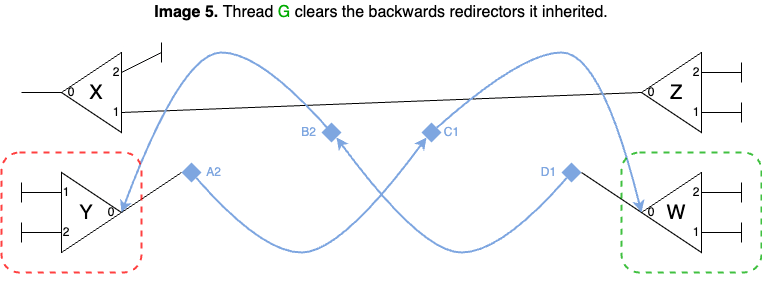
\includegraphics[width=1.0\textwidth,margin=4 4 4 4]{lock_free_evaluator_5.png}
\caption{Lock-free evaluator step 5}
\end{figure}

\begin{figure}[h!]
\centering
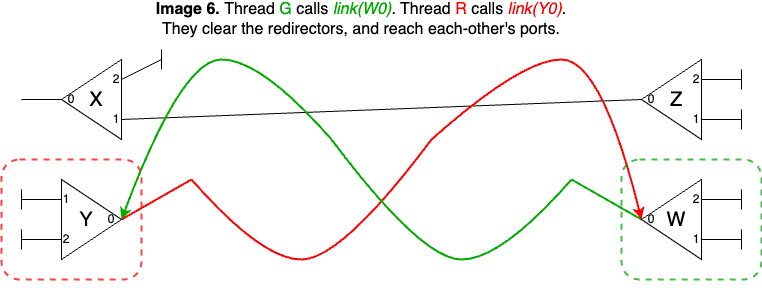
\includegraphics[width=1.0\textwidth,margin=4 4 4 4]{lock_free_evaluator_6.png}
\caption{Lock-free evaluator step 6}
\end{figure}

\begin{figure}[h!]
\centering
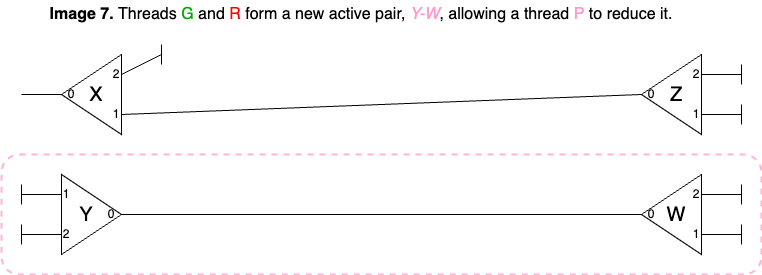
\includegraphics[width=1.0\textwidth,margin=4 4 4 4]{lock_free_evaluator_7.png}
\caption{Lock-free evaluator step 7}
\end{figure}

Note that in Image 2, the reduction is semantically complete, with ports X1-W0 and Y0-Z0 indirectly connected. Each thread independently performs this reduction, without impacting surrounding nodes, by converting the auxiliary ports of their owned nodes to redirectors and then swapping opposing ports (e.g., A1 goes to B1, B2 goes to A2, etc.). This approach entirely avoids locks. The link() procedure in the appendix is then only needed to clear the memory occupied by redirectors and to identify new active pairs. As this clean-up process may cross ownership regions, caution is required to deploy atomics when necessary.

\section{Optimization: 1/4 rewrites}\label{s:lockfree}

The lock-free evaluator procedure above reveals a symmetry that can be exploited to further increase the parallelism of the algorithm. Notice how thread R performs the same logic 4 times:

\begin{itemize}
  \item Move A1 as redirector to B1; if target is main, link B1 towards A1.
  \item Move A2 as redirector to B2; if target is main, link B2 towards A2.
  \item Move B1 as redirector to A1; if target is main, link A1 towards B1.
  \item Move B2 as redirector to A2; if target is main, link A2 towards B2.
\end{itemize}

These 4 segments are, themselves, independent, and can be performed in parallel. This allows a single interaction to be processed by 4 threads, each one performing 1/4 of a rewrite. According to Amdahl's law, the maximum speedup achievable through parallelization is limited by the fraction of the program that must be executed sequentially. By dividing the rewrite process into 4 smaller sequential chunks, we effectively reduce the sequential portion of the algorithm, increasing the maximum potential speedup by 4x. The pseudocode for this optimized approach can be found in the appendix, completing the algorithm and allowing for efficient parallel execution of interaction combinators.

\section{Implementation}\label{s:implementation}

The lock-free evaluator algorithm has been implemented in CUDA~\cite{taelin2022lock} and has successfully reduced large graphs on GPUs with thousands of concurrent threads, suggesting the algorithm's correctness, even though a formal proof is not provided yet. Moreover, our CUDA implementation demonstrates efficient performance, reaching 900 million rewrites per second on an RTX 4090, which is 15 times more than a single-core CPU evaluator. This significant speedup confirms the practical applicability and efficiency of our approach.

\section{Conclusion}\label{s:conclusion}

In this paper, we have presented a lock-free evaluator for interaction combinators that achieves near-ideal speedup on modern GPUs. Our approach leverages the inherent parallelism of interaction combinators and avoids the pitfalls of lock-based evaluators. We also introduced an optimization that further increases the potential for parallelism by breaking down rewrites into smaller sequential chunks. Our CUDA implementation demonstrates the practicality and efficiency of our approach, as well as suggesting its correctness. Future work includes further optimizations, exploring other applications of our lock-free evaluator, and providing formal proofs of correctness.

\begin{thebibliography}{9}
\bibitem{girard1987linear} 
Girard, J. Y. (1987). Linear logic. Theoretical computer science, 50(1), 1-101.

\bibitem{lafont1997interaction} 
Lafont, Y. (1997). Interaction combinators. Information and Computation, 137(1), 69-101.

\bibitem{jiresch2014towards} 
Jiresch, E. (2014). Towards a GPU-based implementation of interaction nets. arXiv preprint arXiv:1404.0076.

\bibitem{mazza2007denotational} 
Mazza, D. (2007). A denotational semantics for the symmetric interaction combinators. Mathematical Structures in Computer Science, 17(3), 527-562.

\bibitem{sato2014implementation}
Sato, S. (2014). Design and implementation of a low-level language for interaction nets. Ph.D. Thesis, University of Sussex.

\bibitem{taelin2022lock} 
Taelin, V. (2022). Higher-order Virtual Machine [Online]. Available at: https://github.com/HigherOrderCO/hvm-core
\end{thebibliography}

\appendix
\section{Pseudocode}\label{app:pseudocode}

In this appendix, we provide the complete pseudocode for the lock-free evaluator algorithm and the 1/4 rewrites optimization.

\begin{lstlisting}
# Atomically links the node in 'src_ref' towards 'dir_ptr'.
def link(src_ref: &Pointer, dir_ptr: Pointer):
  while True:
    # Peek the target, which may not be owned by us.
    trg_ref = dir_ptr.target()
    trg_ptr = trg_ref.read()

    # If target is a redirection, clear and move forward.
    if trg_ptr.is_red():

      # We own the redirection, so we can mutate it.
      trg_ref.write(0)
      dir_ptr = trg_ptr
      continue

    # If target is an aux port, try replacing it with the node.
    elif trg_ptr.is_aux():

      # Peeks the source node.
      src_ptr = src_ref.read()

      # We don't own the port, so we try replacing it.
      if trg_ref.compare_exchange(trg_ptr, src_ptr) == trg_ptr:
        # Collect the orphaned backward path.
        trg_ref = dir_ptr.target()
        trg_ptr = trg_ref.read()
        while trg_ptr.is_red():
          trg_ref.write(0)
          trg_ref = trg_ptr.target()
          trg_ptr = trg_ref.read()

        # Clear source location.
        src_ref.write(0)
        return

      # If the compare_exchange failed, we try again.
      else:
        continue

    # If target is a main port, two threads reach this branch.
    elif trg_ptr.is_nod() or trg_ptr.is_tmp():

      # Sort references, to avoid deadlocks.
      fst_ref, snd_ref = sort(src_ref, trg_ref)

      # Swap the first reference by TMP placeholder.
      fst_ptr = fst_ref.exchange(TMP)

      # First to arrive creates a redex.
      if !fst_ptr.is_tmp():
        snd_ptr = snd_ref.exchange(TMP)
        add_redex(fst_ptr, snd_ptr)
        return

      # Second to arrive clears up the memory.
      else:
        fst_ref.write(0)
        while snd_ref.compare_exchange(snd_ptr, 0) != snd_ptr:
          continue
        return

    # If it is taken, we wait.
    else:
      continue
\end{lstlisting}

\begin{lstlisting}
# Performs 1/4 con-con interaction
def con_con(a_ptr: &Pointer, b_ptr: &Pointer, port: Port):

  # Gets a reference current and opposing ports
  a_aux_ref = &a_ptr.port[port]
  b_aux_ref = &b_ptr.port[port]

  # Takes the current port and casts to redirector
  a_aux_ptr = a_aux_ref.exchange(0).as_redirector()

  # Synchronizes local threads
  local_threads.sync()

  # Sends current port to opposing port
  b_aux_ref.write(a_aux_ptr)

  # Synchronizes local threads
  local_threads.sync()

  # If the current port targeted a main port...
  if a_aux_ptr.targets_main():

    # Link the opposing port towards the current port
    link(b_aux_ref, new_ptr_to(a_aux_ptr))

# Performs 1/4 con-dup interaction
def con_dup(a_ptr: &Pointer, b_ptr: &Pointer, port: Port):
  
  # Gets reference to both aux ptrs
  a_aux_ref = &a_ptr.port[port]
  b_aux_ref = &b_ptr.port[port]

  # Takes my aux ptr
  a_aux_ptr = a_aux_ref.exchange(0).as_redirector()

  # Allocates a new clone
  clone_loc = malloc(1 * size(Ptr))
  clone_ptr = mkptr(a_ptr.tag(), clone_loc)

  # Synchronizes local threads
  local_threads.sync()

  # Communicates this clone's loc to local threads
  local_threads.send_clone_loc(clone_loc)

  # Synchronizes local threads
  local_threads.sync()

  # Gets opposing clone locs
  clone_x_loc, clone_y_loc = local_threads.receive_clone_locs()

  # Fills clone inner wires
  clone_loc[1] = clone_x_loc
  clone_loc[2] = clone_y_loc

  # Sends clone to opposing port
  b_aux_ref.write(clone_ptr)

  # Synchronizes local threads
  local_threads.sync()

  # If the current port targeted an aux port...
  if a_aux_ptr.targets_aux():

    # Link the current port towards its former target
    link(a_aux_ref, a_aux_ptr)

  # If the current port targeted a main port...
  if a_aux_ptr.is_main():

    # Form a new redex between its former and current target
    create_redex(a_aux_ptr, a_aux_ref.exchange(0))
\end{lstlisting}

\begin{lstlisting}
def rewrite(net):
  # Performs each interaction, in parallel
  p-for (a,b) in net.redexes:

    # Sets up the 1/4 interactions
    quarters = [(a,b,1), (a,b,2), (b,a,1), (b,a,2)]

    # Performs each 1/4 interaction, in parallel
    p-for (a, b, port) in quarters:
      match (a_ptr.tag(), b_ptr.tag()):
        (CON, CON) => con_con(a, b, port)
        (CON, DUP) => con_dup(a, b, port)
        (CON, ERA) => con_era(a, b, port)
        (DUP, CON) => dup_con(b, a, port)
        (DUP, DUP) => dup_dup(b, b, port)
        (DUP, ERA) => dup_era(a, b, port)
        (ERA, CON) => era_con(b, a, port)
        (ERA, DUP) => era_dup(b, b, port)
        (ERA, ERA) => era_era(a, b, port)
\end{lstlisting}

\end{document}
